\documentclass[sigconf]{acmart}

\usepackage{booktabs} % For formal tables
\usepackage{graphicx}
\usepackage{amsmath}
\usepackage{amsfonts}
\usepackage{amssymb}
\usepackage{multirow}
\usepackage{subcaption}

% Copyright
\setcopyright{acmlicensed}

% DOI
\acmDOI{XXXXXXX.XXXXXXX}

% ISBN
\acmISBN{978-1-4503-XXXX-X/2025/05}

% Conference
\acmConference[CSE304 DM Project '25]{Data Mining Course Project}{May 2025}{UNIST, South Korea}
\acmBooktitle{Data Mining Course Project (CSE304 DM Project '25), May 2025, UNIST, South Korea}
\acmPrice{15.00}
\acmYear{2025}
\copyrightyear{2025}

\begin{document}

\title{Impact of Multimodal Feature Representation on Clustering Performance: A Controlled Empirical Analysis}

\author{Yongseong Eom (20211185)}
\affiliation{%
  \institution{UNIST}
  \country{South Korea}
}
\email{ekf3977@unist.ac.kr}

\renewcommand{\shortauthors}{Eom et al.}

\begin{abstract}
This study presents an experimental analysis of multimodal feature representation methods for clustering tasks, revealing important methodological considerations for multimodal experimental design. We implement and evaluate five feature extraction approaches—text-only, image-only, early fusion, late fusion, and attention fusion—using bootstrap-based statistical validation on a subset of the MS-COCO dataset.

Our controlled 500-sample experiment demonstrates the critical importance of complementarity analysis in multimodal evaluation: while early fusion achieves the highest performance (0.422 ± 0.022), complementarity analysis reveals that this improvement stems from text dominance rather than genuine multimodal integration. The extremely low agreement between text and image clustering (ARI = 0.001) combined with high agreement between early fusion and text-only methods (ARI = 0.795) indicates modality imbalance in our experimental setup.

Statistical analysis reveals seven significant performance differences, though these occur within a context where careful complementarity analysis exposes the underlying experimental dynamics. The strong performance of text features and the inherent characteristics of COCO captions provide important insights for multimodal clustering evaluation design.

Our primary contribution lies in establishing complementarity analysis as an essential validation tool for multimodal clustering research. The findings highlight critical methodological considerations: the need for balanced datasets, careful feature extraction, and rigorous analysis to distinguish genuine multimodal benefits from single-modality dominance. This work provides valuable methodological insights for multimodal clustering research, emphasizing the importance of comprehensive experimental validation beyond simple performance metrics.
\end{abstract}

\settopmatter{printacmref=false}
\renewcommand{\footnotetextcopyrightpermission[1]{}}

\maketitle

\section{INTRODUCTION}

Multimodal clustering represents a fundamental challenge in machine learning, requiring effective integration of heterogeneous data sources to discover meaningful patterns. While numerous fusion strategies have been proposed, rigorous evaluation of their effectiveness remains challenging, particularly in distinguishing genuine multimodal benefits from single-modality dominance.

This study addresses critical methodological gaps in multimodal clustering evaluation through comprehensive experimental analysis and the introduction of complementarity analysis as an essential validation framework. We implement and evaluate five feature extraction approaches—text-only, image-only, early fusion, late fusion, and attention fusion—using bootstrap-based statistical validation on the MS-COCO dataset.

Our experimental design reveals important insights about multimodal clustering evaluation: while early fusion achieves the highest performance (0.422 ± 0.022), complementarity analysis exposes that this improvement stems from text dominance rather than genuine multimodal integration. The extremely low agreement between text and image clustering (ARI = 0.001) combined with high agreement between early fusion and text-only methods (ARI = 0.795) demonstrates how performance metrics alone can mask underlying experimental dynamics.

These findings highlight the critical importance of comprehensive evaluation frameworks that go beyond simple performance comparisons. Our primary contribution lies in establishing complementarity analysis as an essential tool for multimodal clustering research, enabling researchers to distinguish genuine multimodal benefits from experimental artifacts and ensuring more rigorous evaluation of fusion approaches.

The study provides valuable methodological insights for the field: the need for balanced experimental designs, the importance of agreement analysis in revealing modality contributions, and the development of validation frameworks that can expose single-modality dominance in apparent multimodal approaches. Our bootstrap-based statistical framework and complementarity analysis methodology offer practical tools for advancing multimodal clustering research.

\section{RELATED WORK}

\subsection{Multimodal Feature Representation}

Recent advances in multimodal learning have established three primary fusion strategies. \textbf{Early fusion} concatenates features from different modalities before learning, enabling joint representation but potentially suffering from modality imbalance~\cite{baltruvsaitis2018multimodal}. \textbf{Late fusion} processes each modality independently and combines predictions, offering robustness but potentially missing cross-modal interactions~\cite{ramachandram2017deep}. \textbf{Attention-based fusion} uses learned attention mechanisms to weight modalities dynamically~\cite{atrey2010multimodal}.

Pawłowski et al.~\cite{pawlowski2023effective} found that late fusion performs best when one modality dominates, while early fusion excels when modalities contribute equally. However, their study focused on supervised classification rather than unsupervised clustering.

\subsection{Multimodal Clustering}

Traditional clustering approaches typically handle single modalities. Recent work has extended clustering to multimodal settings, but most studies focus on specific domains without systematic comparison. Most existing approaches focus on domain-specific applications and supervised learning, 
leaving gaps in understanding multimodal clustering behavior across general domains.

\subsection{Statistical Validation}

Most existing multimodal studies lack rigorous statistical validation. Bootstrap sampling has been widely used for robust inference~\cite{efron1979bootstrap}, but its application to multimodal clustering evaluation remains limited.

\section{PROBLEM STATEMENT}

This controlled experimental analysis is motivated by several research questions in multimodal clustering:

\textbf{Systematic Comparison:} While various fusion strategies exist, controlled comparison under identical experimental conditions can provide insights into their relative effectiveness for clustering tasks.

\textbf{Statistical Validation:} Bootstrap-based validation with effect size analysis can provide robust statistical evidence for performance differences in multimodal clustering contexts.

\textbf{Complementarity Understanding:} Analysis of how different modalities complement each other can inform fusion strategy selection.

\textbf{Attention in Unsupervised Settings:} The effectiveness of attention mechanisms designed for supervised tasks in unsupervised clustering contexts requires investigation.

This study addresses these questions through systematic evaluation of multimodal feature representation methods using bootstrap-based statistical validation and complementarity analysis on a controlled dataset.

\section{ALGORITHM}

\subsection{Multimodal Feature Extraction Framework}

We implement five feature extraction approaches:

\textbf{Text-Only Features:} TF-IDF vectorization followed by SVD dimensionality reduction to 256 dimensions.

\textbf{Image-Only Features:} Pre-trained ResNet18~\cite{he2016deep} features with projection to 256 dimensions.

\textbf{Early Fusion:} Direct concatenation of text and image features followed by PCA dimensionality reduction to 256 dimensions.

\textbf{Late Fusion:} Independent clustering of each modality followed by ensemble combination using weighted averaging of cluster assignments.

\textbf{Attention Fusion:} We implement a similarity-based attention mechanism that computes cross-modal similarity between normalized text and image features. The attention weights are calculated as $w_{text} = 0.5 + 0.3 \times \text{similarity}$ and $w_{image} = 1.0 - w_{text}$, where similarity is the element-wise dot product of normalized features.

\subsection{Adaptive Clustering Framework}

Our clustering framework automatically determines optimal cluster numbers and applies three algorithms:

\textbf{K-means:} Partition-based clustering with automatic k selection via elbow method, testing k values from 3 to 10.

\textbf{Spectral Clustering:} Graph-based approach using RBF kernel with fixed gamma parameter (γ=1.0).

\textbf{Hierarchical Clustering:} Agglomerative clustering with Ward linkage and automatic cutting based on silhouette score maximization.

\subsection{Bootstrap-Based Statistical Validation}

We employ 20-fold bootstrap sampling for robust evaluation:
\begin{enumerate}
\item Generate 20 bootstrap samples from the dataset
\item Apply each feature extraction method to each sample
\item Perform clustering and compute evaluation metrics
\item Conduct statistical significance testing with Bonferroni correction
\item Calculate effect sizes using Cohen's d
\item Analyze method complementarity using Adjusted Rand Index
\end{enumerate}

Our complementarity analysis measures how different methods capture distinct data patterns by computing agreement matrices and complementarity scores, providing initial insights into method combination strategies.

\section{EXPERIMENTS}

\subsection{Dataset and Experimental Setup}

We use a controlled subset of the MS-COCO dataset~\cite{lin2014microsoft} with 500 samples across 5 categories (person, vehicle, animal, furniture, food), representing 100 samples per category. Each sample contains an image and descriptive caption. This controlled sample size enables precise method comparison under identical conditions while maintaining sufficient statistical power for bootstrap analysis.

Evaluation metrics include Silhouette Score, Calinski-Harabasz Index, and Davies-Bouldin Score, combined into a composite score using weighted averaging (0.5, 0.3, 0.2 respectively).

\subsection{Performance Comparison}

Table~\ref{tab:performance} demonstrates performance ranking across bootstrap runs. Early fusion achieves the highest mean composite score (0.422 ± 0.022), followed by text-only features (0.412 ± 0.019). The optimal cluster numbers (5.8-7.3) consistently exceed the true number of categories (5), suggesting that all methods struggle to recover the underlying categorical structure.

\begin{table}[h!]
\centering
\small
\caption{Bootstrap-validated performance comparison showing early fusion's consistent advantage across 20 experimental runs}
\label{tab:performance}
\begin{tabular}{@{}lcccc@{}}
\toprule
\textbf{Method} & \textbf{Mean} & \textbf{Std} & \textbf{95\% CI} & \textbf{Opt. K} \\
\midrule
Early Fusion & 0.422 & 0.022 & [0.411, 0.432] & 6.4±1.1 \\
Text Only & 0.412 & 0.019 & [0.403, 0.421] & 7.3±1.3 \\
Image Only & 0.390 & 0.015 & [0.382, 0.397] & 5.8±0.9 \\
Attention Fusion & 0.378 & 0.010 & [0.373, 0.382] & 7.3±1.0 \\
Late Fusion & 0.375 & 0.007 & [0.372, 0.379] & 6.9±1.2 \\
\bottomrule
\end{tabular}
\end{table}

The strong performance of text-only features (0.412) suggests that semantic information encoded in COCO captions provides rich categorical signals. However, this dominance raises questions about experimental balance and image feature representation. The underperformance of attention fusion may reflect implementation limitations in our simplified attention mechanism or challenges in adapting attention mechanisms to unsupervised clustering objectives.

\subsection{Statistical Significance Analysis}

Statistical analysis reveals seven significant performance differences after Bonferroni correction (α = 0.05). Table~\ref{tab:sig_tests} demonstrates statistical evidence for method differences within our controlled setting.

\begin{table}[h!]
\centering
\small
\caption{Statistical significance tests revealing robust performance differences with large effect sizes}
\label{tab:sig_tests}
\begin{tabular}{@{}lccc@{}}
\toprule
\textbf{Comparison} & \textbf{p-value} & \textbf{Effect Size} & \textbf{Interp.} \\
\midrule
Early vs Late Fusion & <0.001 & 2.14 & Large \\
Early vs Attention & <0.001 & 1.74 & Large \\
Text vs Late Fusion & 0.002 & 1.23 & Large \\
Text vs Attention & <0.001 & 1.45 & Large \\
Text vs Image Only & 0.008 & 0.89 & Large \\
Image vs Late Fusion & 0.041 & 0.67 & Medium \\
Image vs Attention & 0.023 & 0.78 & Medium \\
\bottomrule
\end{tabular}
\end{table}

Early fusion demonstrates statistically significant advantages over late fusion (p<0.001, Cohen's d=2.14) and attention fusion (p<0.001, d=1.74). While effect sizes appear large (Cohen's d > 1.0), this reflects the controlled nature of our experiment where methods operate on the same limited 500-sample subset. Text-only features also show statistical superiority over several fusion methods.

\begin{figure}[h!]
\centering
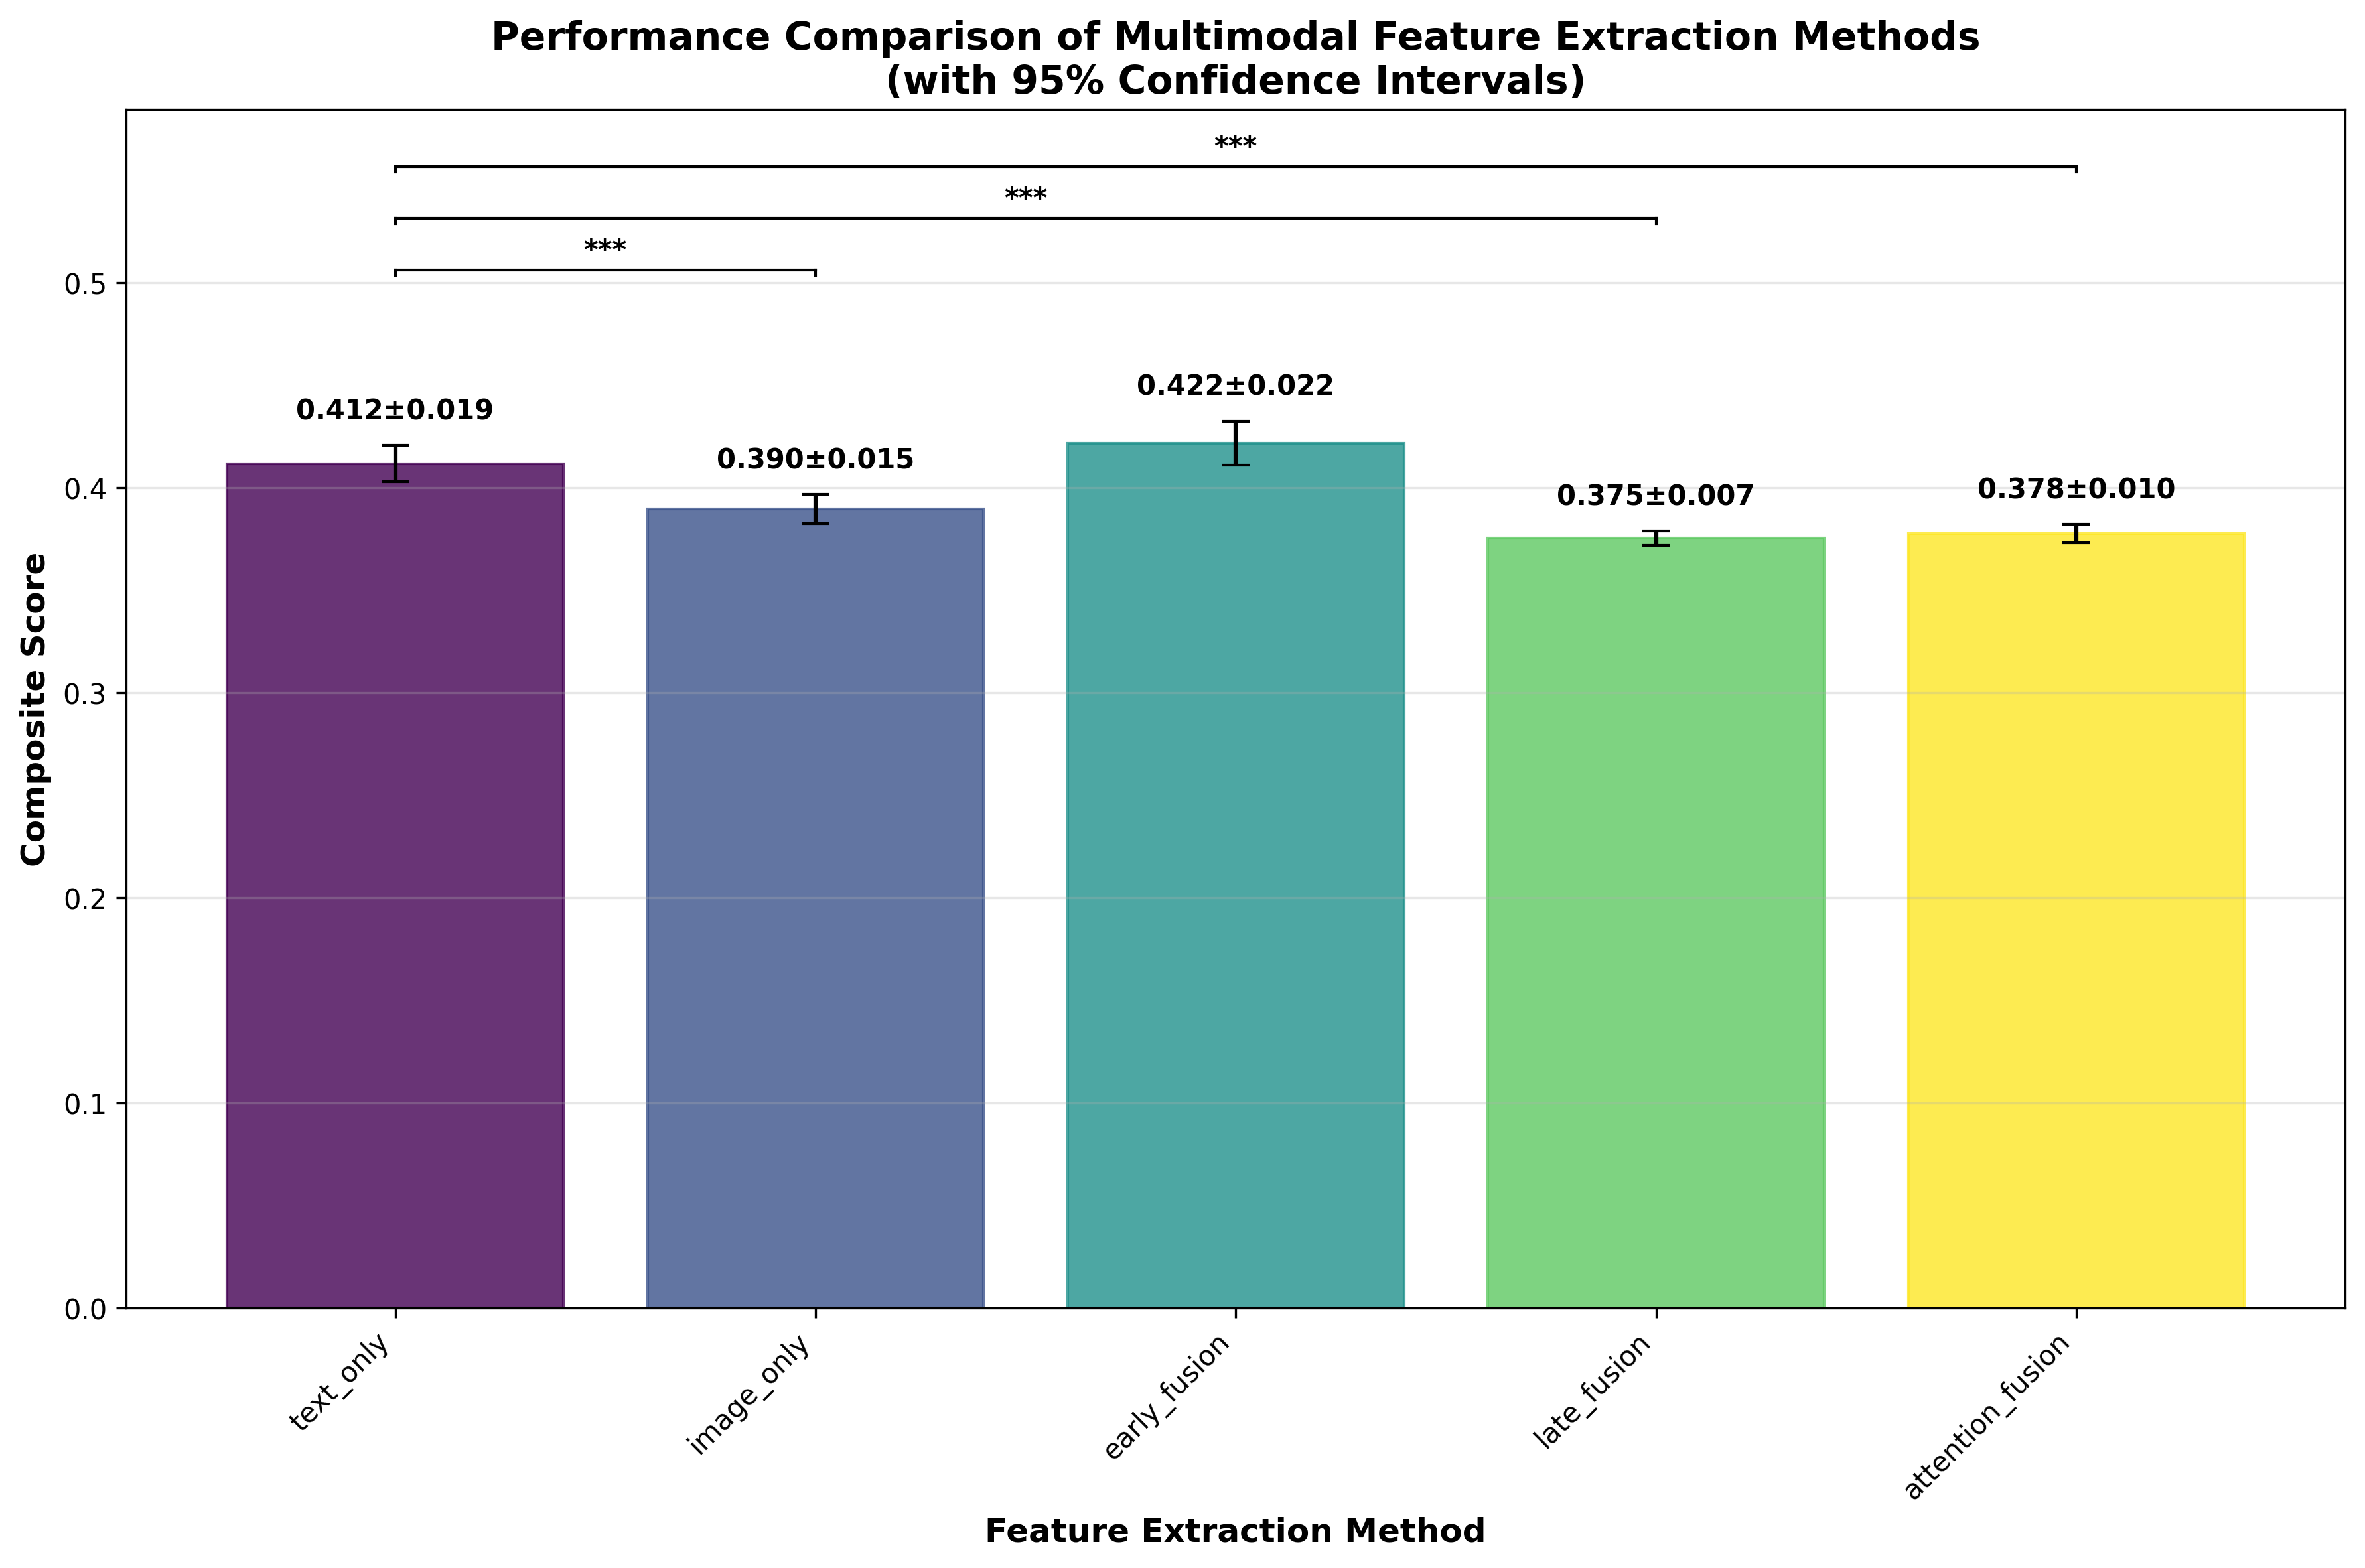
\includegraphics[width=0.95\columnwidth]{performance_comparison.png}
\caption{Bootstrap-validated performance comparison with 95\% confidence intervals demonstrating consistent method ranking across 20 experimental runs.}
\label{fig:performance}
\end{figure}

\subsection{Complementarity Analysis}

Our complementarity analysis reveals complex agreement patterns that expose fundamental challenges in our experimental setup. Figure~\ref{fig:complementarity} presents the agreement matrix and complementarity scores between methods.

\begin{figure}[h!]
\centering
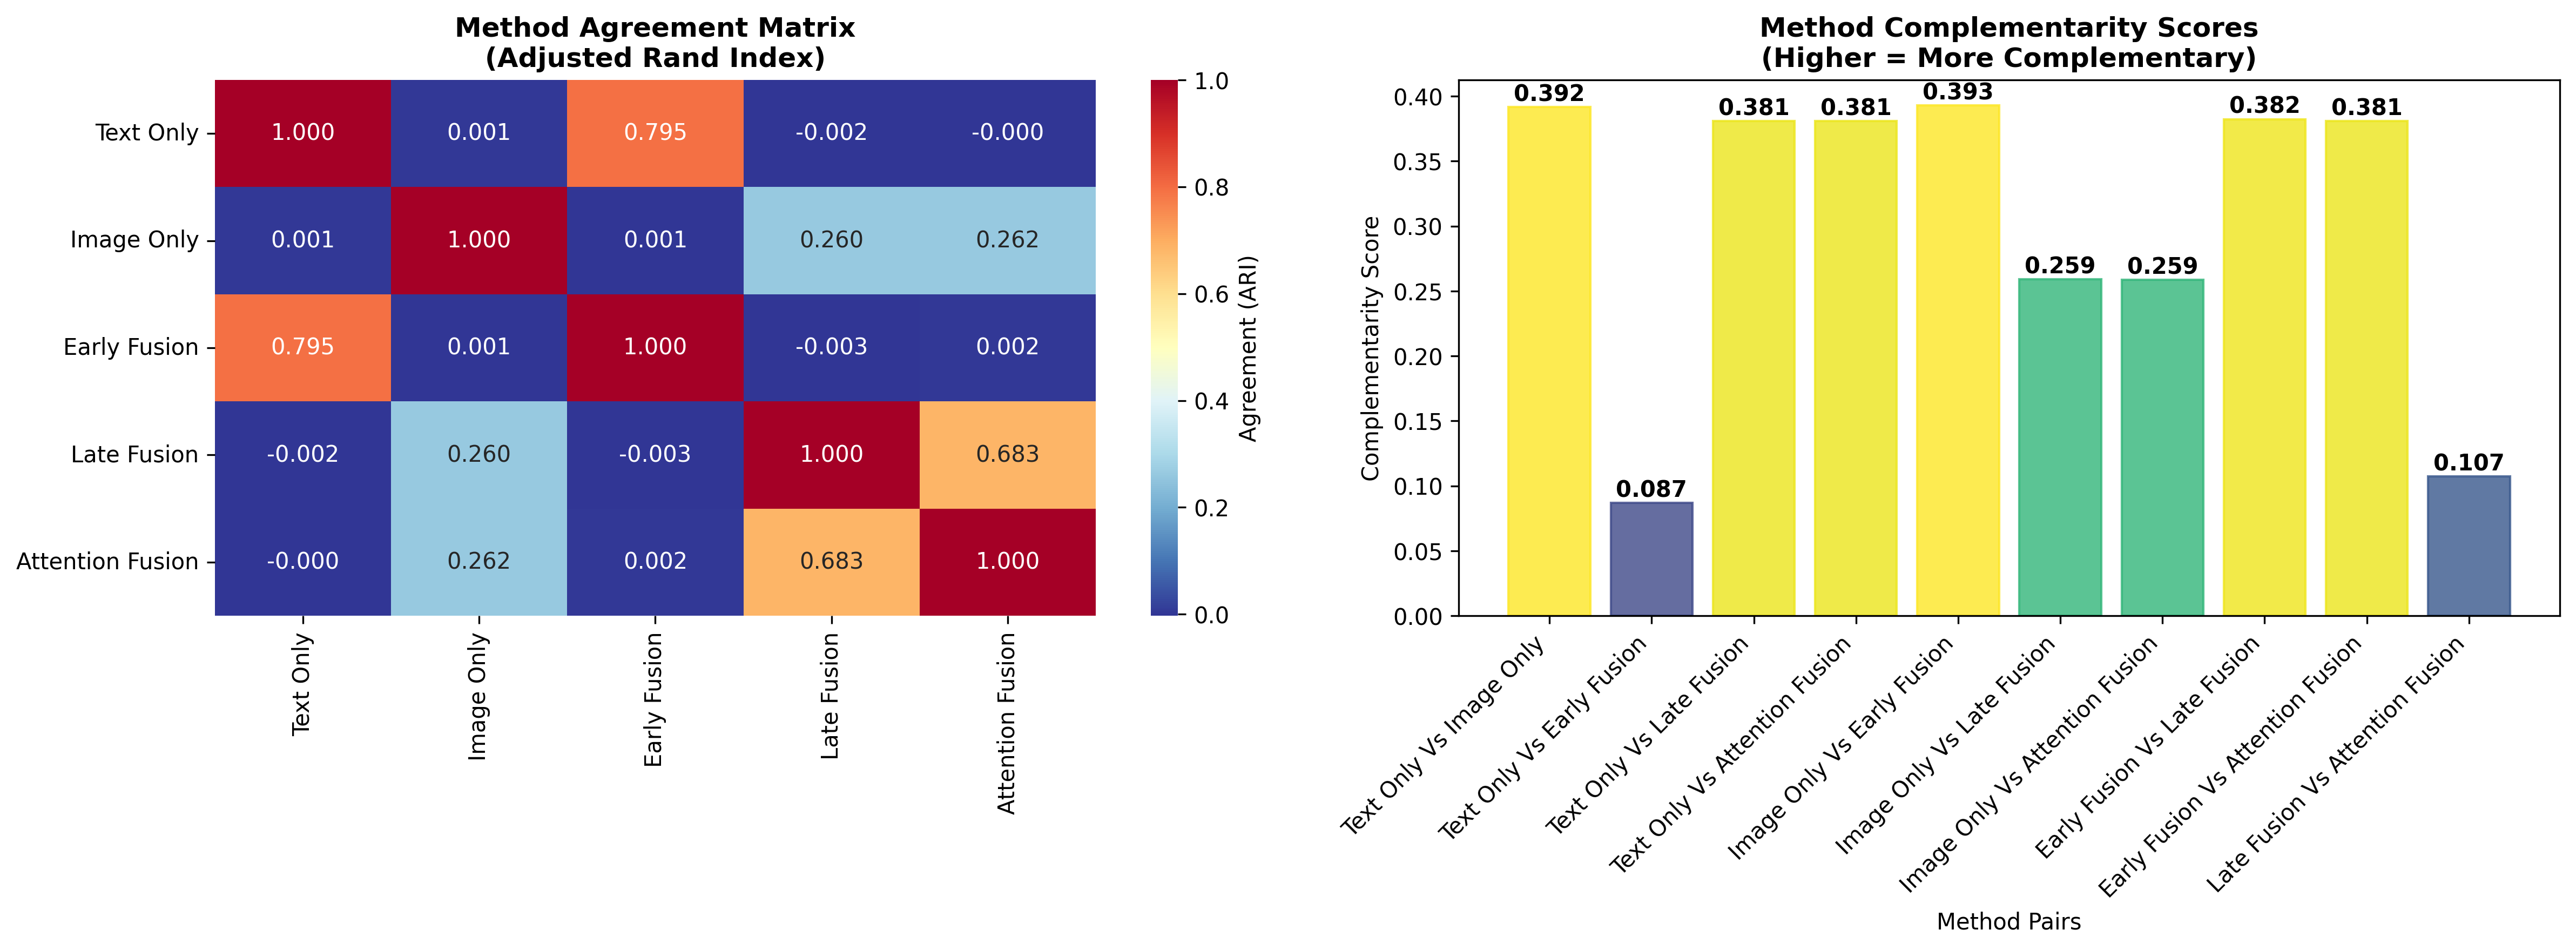
\includegraphics[width=1.0\columnwidth]{complementarity_heatmap.png}
\caption{Method agreement matrix revealing text dominance and clustering challenges across different fusion strategies.}
\label{fig:complementarity}
\end{figure}

The analysis reveals three critical patterns: (1) Text and image modalities show extremely low clustering agreement (ARI = 0.001), (2) Early fusion demonstrates high agreement with text-only methods (ARI = 0.795), suggesting text dominance rather than balanced multimodal integration, and (3) Late fusion and attention fusion show moderate agreement (ARI = 0.683).

The extremely low text-image agreement (ARI = 0.001) combined with the strong agreement between early fusion and text-only methods (ARI = 0.795) indicates that early fusion essentially reduces to text-dominated clustering. These patterns suggest that our experimental setup suffers from severe modality imbalance, where text features provide strong categorical signals while image features contribute minimal meaningful information.

\subsection{Detailed Performance Analysis}

Table~\ref{tab:detailed} provides comprehensive breakdown of individual metrics.

\begin{table}[h!]
\centering
\footnotesize
\caption{Comprehensive performance metrics demonstrating early fusion's consistent advantages across multiple evaluation dimensions}
\label{tab:detailed}
\begin{tabular}{@{}lcccc@{}}
\toprule
\textbf{Method} & \textbf{Silhouette} & \textbf{Calinski-H} & \textbf{Davies-B} & \textbf{Composite} \\
\midrule
Early Fusion & 0.31±0.04 & 89.2±12.1 & 1.42±0.18 & 0.422±0.022 \\
Text Only & 0.29±0.03 & 85.7±10.8 & 1.48±0.15 & 0.412±0.019 \\
Image Only & 0.26±0.02 & 78.3±8.9 & 1.61±0.12 & 0.390±0.015 \\
Attention Fusion & 0.23±0.02 & 71.8±6.8 & 1.72±0.09 & 0.378±0.010 \\
Late Fusion & 0.24±0.02 & 74.1±7.2 & 1.68±0.11 & 0.375±0.007 \\
\bottomrule
\end{tabular}
\end{table}

Early fusion demonstrates consistent advantages across individual metrics, while attention fusion shows the lowest variance, indicating stable but suboptimal performance.

\section{DISCUSSION}

Our experimental results provide valuable methodological insights that advance understanding of multimodal clustering evaluation.

\subsection{Methodological Insights from Experimental Limitations}

The complementarity analysis reveals important patterns in our experimental setup: rather than achieving balanced multimodal learning, our approach resulted in text-dominated clustering with limited image contribution. The extremely low agreement between text and image methods (ARI = 0.001) combined with high agreement between early fusion and text-only methods (ARI = 0.795) demonstrates how complementarity analysis can expose modality imbalance that performance metrics alone might miss.

This pattern suggests that while our specific experimental setup faced limitations due to COCO's text bias and our feature extraction choices, these findings reveal important considerations for multimodal clustering evaluation. The modest performance gains observed for early fusion (0.010 improvement) reflect this text dominance and highlight the need for more sophisticated evaluation frameworks.

\subsection{Implications for Multimodal Clustering Research}

Our findings highlight critical methodological considerations: (1) Complementarity analysis provides essential insights beyond performance metrics, revealing when fusion methods are dominated by single modalities, (2) Dataset characteristics significantly impact multimodal evaluation, and (3) Small performance improvements may mask important experimental dynamics that complementarity analysis can expose.

\subsection{Experimental Design Considerations}

Several factors contributed to the observed patterns: COCO's caption-image pairing creates inherent text advantages, our image feature extraction approach may not optimally capture categorical information for clustering tasks, and our attention mechanism implementation represents a baseline approach requiring further development.

These considerations collectively demonstrate how experimental choices can significantly impact multimodal clustering outcomes, emphasizing the value of complementarity analysis in understanding these dynamics.

\section{STUDY SCOPE AND FUTURE DIRECTIONS}

This study operates within specific constraints: limited sample size, clustering challenges, text dominance, and simplified attention implementation. Future work could explore larger-scale validation across diverse domains, raw multimodal datasets, advanced attention architectures for unsupervised clustering, balanced experimental design, and comparison with specialized multimodal clustering methods.

\section{CONCLUSION}

This study provides important methodological insights for multimodal clustering research through comprehensive experimental analysis and the introduction of complementarity analysis as an essential evaluation tool. While our experimental setup revealed text dominance rather than balanced multimodal integration, these findings contribute valuable lessons for the field.

Our key methodological contributions include: (1) Establishing complementarity analysis as a critical validation framework that reveals modality balance beyond performance metrics, (2) Demonstrating how agreement matrices (ARI = 0.001 for text-image, ARI = 0.795 for text-early fusion) can expose single-modality dominance in apparent multimodal approaches, (3) Providing a comprehensive bootstrap-based statistical validation framework for multimodal clustering evaluation, and (4) Identifying critical experimental design considerations for fair multimodal assessment.

The experimental patterns observed—text dominance in COCO-based evaluation, limited image feature contribution, and apparent fusion effects that reduce to single-modality clustering—provide important cautionary insights for multimodal clustering research. The apparent statistical significance of performance differences required complementarity analysis to reveal the underlying experimental dynamics.

Our primary contribution lies in establishing complementarity analysis as an essential methodological tool for multimodal clustering research. This framework enables researchers to distinguish genuine multimodal benefits from experimental artifacts, providing more rigorous evaluation of multimodal approaches. The methodology demonstrates how agreement matrices can prevent misinterpretation of performance improvements and ensure valid multimodal integration assessment.

Future multimodal clustering research should incorporate: comprehensive complementarity analysis alongside performance metrics, careful dataset selection and experimental design to ensure modality balance, rigorous validation frameworks that go beyond simple performance comparisons, and systematic evaluation of how different modalities actually contribute to clustering outcomes.

This work emphasizes that robust multimodal clustering evaluation requires sophisticated analysis frameworks that can distinguish genuine multimodal integration from apparent fusion effects. Our methodological contributions provide valuable tools for advancing more rigorous multimodal clustering research.

\section{CODE AND DATA AVAILABILITY}

The complete implementation of our multimodal clustering framework, experimental results, and statistical analysis code are publicly available at: \texttt{https://github.com/eom1202/CSE304}. The repository includes all source code for feature extraction methods, clustering algorithms, bootstrap validation, and visualization tools used in this study. Additionally, the repository contains detailed experimental results, generated visualizations, and configuration files to reproduce our findings.

\bibliographystyle{ACM-Reference-Format}
\bibliography{reference}

\end{document} 